\documentclass{beamer}
\usepackage{amsmath}
\usepackage[english]{babel} %set language; note: after changing this, you need to delete all auxiliary files to recompile
\usepackage[utf8]{inputenc} %define file encoding; latin1 is the other often used option
\usepackage{csquotes} % provides context sensitive quotation facilities
\usepackage{graphicx} %allows for inserting figures
\usepackage{booktabs} % for table formatting without vertical lines
\usepackage{textcomp} % allow for example using the Euro sign with \texteuro
\usepackage{stackengine}
\usepackage{wasysym}
\usepackage{tikzsymbols}
\usepackage{textcomp}
\usepackage{xcolor}
\usepackage[dvipsnames]{xcolor}
\usepackage{colortbl}
\usepackage{adjustbox}
\usetikzlibrary{decorations.pathreplacing}
\newcommand{\bubblethis}[2]{
        \tikz[remember picture,baseline]{\node[anchor=base,inner sep=0,outer sep=0]%
        (#1) {\underline{#1}};\node[overlay,cloud callout,callout relative pointer={(0.2cm,-0.7cm)},%
        aspect=2.5,fill=yellow!90] at ($(#1.north)+(-0.5cm,1.6cm)$) {#2};}%
    }%
\tikzset{face/.style={shape=circle,minimum size=4ex,shading=radial,outer sep=0pt,
        inner color=white!50!yellow,outer color= yellow!70!orange}}
%% Some commands to make the code easier
\newcommand{\emoticon}[1][]{%
  \node[face,#1] (emoticon) {};
  %% The eyes are fixed.
  \draw[fill=white] (-1ex,0ex) ..controls (-0.5ex,0.2ex)and(0.5ex,0.2ex)..
        (1ex,0.0ex) ..controls ( 1.5ex,1.5ex)and( 0.2ex,1.7ex)..
        (0ex,0.4ex) ..controls (-0.2ex,1.7ex)and(-1.5ex,1.5ex)..
        (-1ex,0ex)--cycle;}
\newcommand{\pupils}{
  %% standard pupils
  \fill[shift={(0.5ex,0.5ex)},rotate=80] 
       (0,0) ellipse (0.3ex and 0.15ex);
  \fill[shift={(-0.5ex,0.5ex)},rotate=100] 
       (0,0) ellipse (0.3ex and 0.15ex);}

\newcommand{\emoticonname}[1]{
  \node[below=1ex of emoticon,font=\footnotesize,
        minimum width=4cm]{#1};}
\usepackage{scalerel}
\usetikzlibrary{positioning}
\usepackage{xcolor,amssymb}
\newcommand\dangersignb[1][2ex]{%
  \scaleto{\stackengine{0.3pt}{\scalebox{1.1}[.9]{%
  \color{red}$\blacktriangle$}}{\tiny\bfseries !}{O}{c}{F}{F}{L}}{#1}%
}
\newcommand\dangersignw[1][2ex]{%
  \scaleto{\stackengine{0.3pt}{\scalebox{1.1}[.9]{%
  \color{red}$\blacktriangle$}}{\color{white}\tiny\bfseries !}{O}{c}{F}{F}{L}}{#1}%
}
\usepackage{fontawesome} % Social Icons
\usepackage{epstopdf} % allow embedding eps-figures
\usepackage{tikz} % allows drawing figures
\usepackage{amsmath,amssymb,amsthm} %advanced math facilities
\usepackage{lmodern} %uses font that support italic and bold at the same time
\usepackage{hyperref}
\usepackage{tikz}
\hypersetup{
    colorlinks=true,
    linkcolor=blue,
    filecolor=magenta,      
    urlcolor=blue,
}
\usepackage{tcolorbox}
%add citation management using BibLaTeX
\usepackage[citestyle=authoryear-comp, %define style for citations
    bibstyle=authoryear-comp, %define style for bibliography
    maxbibnames=10, %maximum number of authors displayed in bibliography
    minbibnames=1, %minimum number of authors displayed in bibliography
    maxcitenames=3, %maximum number of authors displayed in citations before using et al.
    minnames=1, %maximum number of authors displayed in citations before using et al.
    datezeros=false, % do not print dates with leading zeros
    date=long, %use long formats for dates
    isbn=false,% show no ISBNs in bibliography (applies only if not a mandatory field)
    url=false,% show no urls in bibliography (applies only if not a mandatory field)
    doi=false, % show no dois in bibliography (applies only if not a mandatory field)
    eprint=false, %show no eprint-field in bibliography (applies only if not a mandatory field)
    backend=biber %use biber as the backend; backend=bibtex is less powerful, but easier to install
    ]{biblatex}
\addbibresource{../mybibfile.bib} %define bib-file located one folder higher


\usefonttheme[onlymath]{serif} %set math font to serif ones

\definecolor{beamerblue}{rgb}{0.2,0.2,0.7} %define beamerblue color for later use

%%% defines highlight command to set text blue
\newcommand{\highlight}[1]{{\color{blue}{#1}}}


%%%%%%% commands defining backup slides so that frame numbering is correct

\newcommand{\backupbegin}{
   \newcounter{framenumberappendix}
   \setcounter{framenumberappendix}{\value{framenumber}}
}
\newcommand{\backupend}{
   \addtocounter{framenumberappendix}{-\value{framenumber}}
   \addtocounter{framenumber}{\value{framenumberappendix}}
}

%%%% end of defining backup slides

%Specify figure caption, see also http://tex.stackexchange.com/questions/155738/caption-package-not-working-with-beamer
\setbeamertemplate{caption}{\insertcaption} %redefines caption to remove label "Figure".
%\setbeamerfont{caption}{size=\scriptsize,shape=\itshape,series=\bfseries} %sets figure  caption bold and italic and makes it smaller


\usetheme{Boadilla}

%set options of hyperref package
\hypersetup{
    bookmarksnumbered=true, %put section numbers in bookmarks
    naturalnames=true, %use LATEX-computed names for links
    citebordercolor={1 1 1}, %color of border around cites, here: white, i.e. invisible
    linkbordercolor={1 1 1}, %color of border around links, here: white, i.e. invisible
    colorlinks=true, %color links
    anchorcolor=black, %set color of anchors
    linkcolor=beamerblue, %set link color to beamer blue
    citecolor=blue, %set cite color to beamer blue
    pdfpagemode=UseThumbs, %set default mode of PDF display
    breaklinks=true, %break long links
    pdfstartpage=1 %start at first page
    }


\newtcolorbox{boxA}{
    fontupper = \bf,
    boxrule = 1.5pt,
    colframe = black % frame color
}
\newtcolorbox{boxB}{
    boxrule = 1.5pt,
    colframe = blue!70!black,, % frame color
    colback = blue!7!white,
}

% --------------------
% Overall information
% --------------------
\title[Economía I]{Economía I \vspace{3mm}
\\ Magistral 22 \vspace{3mm} \\ Mercado de Trabajo}
\date{}
\author[Victoria Rosino]{Victoria Rosino}
\vspace{0.3cm}
\institute[]{Universidad de San Andrés} 

\begin{document}

\begin{frame}
\vspace{0.3cm}
\titlepage
\centering
\vspace{-0.9cm}
\includegraphics[scale=0.3]{Slides Principios de Economia/Figures/udesa_logo.jpg} 
\end{frame}

\begin{frame}{Mercado de Trabajo: conceptos claves}
    \vspace{0.3cm}
    \textbf{Oferta de trabajo: ¿Quiénes ofrecen trabajo?}
    \begin{itemize}
        \item Personas que buscan activamente empleo o están dispuestas a trabajar.
        \item La oferta puede medirse en cantidad de trabajadores o en horas totales ofrecidas.
    \end{itemize}

    \vspace{0.3cm}

    \textbf{Demanda de trabajo: ¿Quiénes demandan trabajo?}
    \begin{itemize}
        \item Empresas, organizaciones y particulares que desean contratar empleados o comprar horas de trabajo.
        \item Depende principalmente del valor que genera cada trabajador adicional para la producción (productividad marginal).
    \end{itemize}

    \vspace{0.3cm}

    \textbf{Salario:} es el precio del trabajo (puede ser nominal o real).
\end{frame}

\begin{frame}{Mercado de Trabajo: supuestos}
    \vspace{0.3cm}
    \begin{itemize}
        \item Vamos a considerar que la demanda y la oferta se definen en términos de la \textbf{cantidad de empleados} ($T)$. \vspace{0.2cm}
        \item El salario $W$ es el salario nominal, mientras que $w$ es el salario real ($w=W/P$).  \vspace{0.1cm}
        \begin{itemize}
        \item El \textbf{salario nominal} es el sueldo "en el bolsillo". \vspace{0.1cm}
        \item El \textbf{salario real} es cuánto dinero recibe el trabajador en términos de bienes (poder adquisitivo). \vspace{0.1cm}
        \item Vamos a modelar gráficamente usando el salario nominal ($W$). Es decir, a lo largo de una curva de demanda y oferta de trabajo, los precios se mantienen fijos. 
    \end{itemize}
    \end{itemize}


\end{frame}


\begin{frame}{Demanda de trabajo}
    \footnotesize
    \textbf{La demanda de trabajo depende de:}
    \begin{itemize}
        \item \textbf{Salario} ($W$): costo de contratación para los empleadores.
        \item \textbf{Precio} ($P$): el precio de los bienes y servicios que producen las empresas.
        \item \textbf{Productividad marginal del trabajo} ($PMgT$): cuánta producción adicional genera cada trabajador contratado.
    \end{itemize}
    \centering
    \vspace{0.2cm}
    \begin{minipage}{0.55\textwidth}
        \begin{center}
            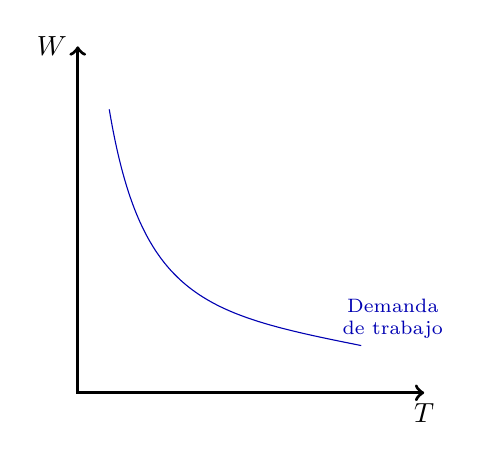
\begin{tikzpicture}[scale=0.4]
            \draw[very thick,<->] (0,11) node[left]{$W$}--(0,0)--(11,0) node[below]{$T$};
            \draw[thin, blue!70!black] (1,9).. controls (2,3) and (4, 2.5) .. (9, 1.5);
            \node [blue!70!black] at (10,2.75) {\scriptsize Demanda};
            \node [blue!70!black] at (10,2) {\scriptsize de trabajo};
            \end{tikzpicture}
        \end{center}
    \end{minipage}
\begin{minipage}{0.4\textwidth}
        Las empresas comparan el salario ($W$) con el valor que aporta un trabajador adicional ($P\times PMgT$). Como $PMgT$ es decreciente, la \textbf{pendiente} de la curva de demanda es \textbf{negativa}. 
\end{minipage}

\end{frame}


\begin{frame}{Demanda de trabajo}

    \begin{itemize}
        \item ¿Qué pasa si aumentan los precios? 
        \item Si los precios suben $x\%$, la demanda de trabajo se desplaza un $x\%$ hacia arriba: los empresarios estarán dispuestos a pagar un mayor salario \underline{nominal} porque lo que venden vale más. 
        \item Esto genera que, para una cantidad contratada $T_d$, el salario \underline{real} se mantenga igual.
    \end{itemize}
        \begin{center}
            \begin{figure}[H]
            \begin{center}
            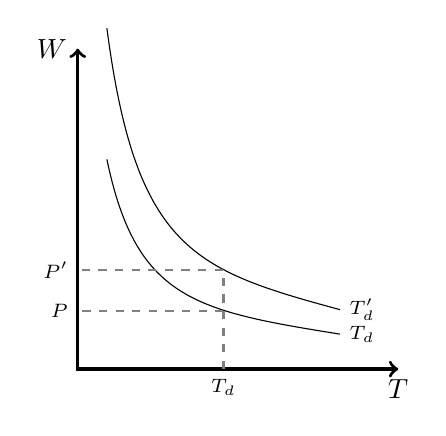
\begin{tikzpicture}[scale=0.37]
            \draw[very thick,<->] (0,11) node[left]{$W$}--(0,0)--(11,0) node[below]{$T$};
            \draw[thin] (1,7.2).. controls (2,2.4) and (4, 2) .. (9, 1.2) node [right] {\scriptsize $T_d$};
            \draw[thin] (1,11.7).. controls (2,4.08) and (4, 3.4) .. (9, 2.04) node [right] {\scriptsize$T_d'$}; 
            \draw[thick,gray,dashed](5,0)--(5,3.4)--(0,3.4);
            \draw[thick,gray,dashed](5,2)--(0,2);
            \node[left] at (0,2) {\scriptsize $P$};
            \node[left] at (0,3.4) {\scriptsize $P'$};
            \node[below] at (5,0) {\scriptsize $T_d$};
            \end{tikzpicture}
            \end{center}
            \end{figure}
        \end{center}
\end{frame}

\begin{frame}{Oferta de trabajo}
\small
\textbf{¿Cómo responde la oferta de trabajo ante cambios en el salario?}
\begin{enumerate}
\item \textbf{Shock transitorio (aumento temporal del salario):}
\begin{itemize}
    \item La oferta de trabajo \textbf{aumenta}.
    \item \textit{Efecto sustitución $>$ Efecto ingreso.}
    \begin{itemize}
        \item El tiempo libre se vuelve más caro $\Rightarrow$ se trabaja más.
        \item No hay tiempo suficiente para “sentirse más rico”.
    \end{itemize}
\end{itemize}

\item \textbf{Shock permanente (aumento sostenido del salario):}
\begin{itemize}
    \item La oferta de trabajo \textbf{no cambia significativamente}.
    \item \textit{Efecto sustitución $\simeq$ Efecto ingreso.}
    \begin{itemize}
        \item Se quiere trabajar más (sustitución).
        \item Pero también disfrutar más ocio (ingreso).
    \end{itemize}
\end{itemize}
\end{enumerate}
\textbf{Ejemplo histórico:}  
Desde la Edad Media, las horas trabajadas por día apenas han bajado (de 9 a 8 horas), a pesar de que los salarios reales aumentaron más de 6000\%. $\Rightarrow$ Elasticidad muy baja.
\end{frame}

\begin{frame}{Oferta de trabajo}
\begin{columns}
\column{0.5\textwidth}

\textbf{Curvas de oferta de trabajo:}
    \small
    \begin{itemize}
        \item \textbf{\textcolor{magenta}{LP (largo plazo):}} La oferta es \textbf{completamente inelástica} a partir de un salario de reserva \(\bar{W}\).
        
        \item \textbf{\textcolor{blue}{CP (corto plazo)}}  
        Un aumento \textbf{transitorio} del salario genera más oferta de trabajo:  
        efecto sustitución \(>\) efecto ingreso.

        \item \textbf{Salario de reserva \(\bar{W}\):}  
        Mínimo salario aceptado para ofrecer trabajo.
    \end{itemize}
    \column{0.5\textwidth}
        \begin{figure}[H]
        \begin{center}
        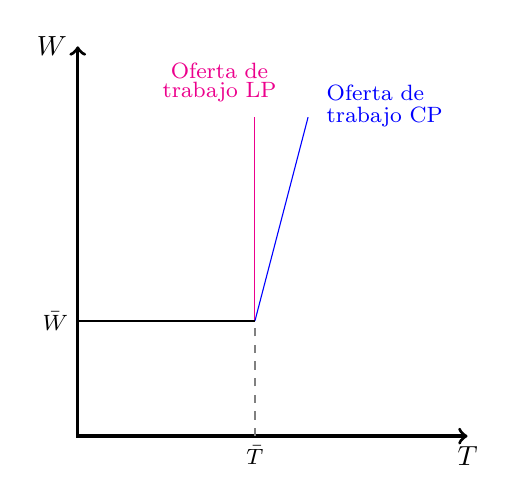
\begin{tikzpicture}[scale=0.45]
        \draw[very thick,<->] (0,11) node[left]{$W$}--(0,0)--(11,0) node[below]{$T$};
        \draw[thin, magenta](5,3.25)--(5,9);
        \node [magenta] at (4,10.3) {\footnotesize Oferta de};
        \node [magenta] at (4,9.7) {\footnotesize  trabajo LP};
        \draw[thin, blue](5,3.25)--(6.5,9);
        \node [right, blue] at (6.75,9.7) {\footnotesize Oferta de};
        \node [right, blue] at (6.75,9) {\footnotesize  trabajo CP};
        \draw[thin](5,3.25)--(0,3.25);
        \node [left] at (0,3.25) {\footnotesize  $\bar{W}$};
        \draw[thick,gray,dashed](5,0)--(5,3.25);
        \node[below] at (5,0) {\footnotesize $\bar{T}$};
        \end{tikzpicture}
        \end{center}
        \end{figure}
    \end{columns}
\end{frame}



\begin{frame}{Mercado de trabajo: el equilibrio}
    \begin{columns}
    \column{0.5\textwidth}
    \footnotesize
    \begin{itemize}
        \item El salario de equilibrio (\(W^*\)) se alcanza cuando la \textbf{cantidad ofrecida} de trabajo coincide con la \textbf{cantidad demandada}.
        
        \item Si el salario es \textbf{mayor que \(W^*\)} (como \(W^{**}\)), las empresas quieren contratar menos trabajadores (\(T_d < T_o\)).

        \item Aparece entonces \textbf{desempleo involuntario}: personas dispuestas a trabajar al salario vigente, pero que no consiguen empleo.

    \end{itemize}

    \column{0.5\textwidth}
        \begin{center}
        \scriptsize
        \begin{figure}[H]
        \begin{center}
        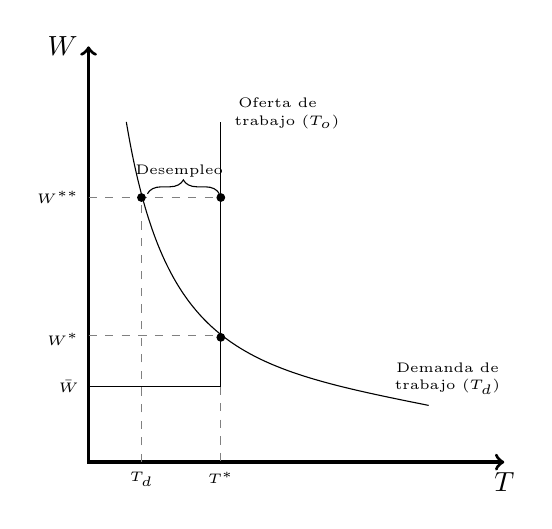
\begin{tikzpicture}[scale=0.48]
        \draw[very thick,<->] (0,11) node[left]{$W$}--(0,0)--(11,0) node[below]{$T$};
        \draw[thin] (1,9).. controls (2,3) and (4, 2.5) .. (9, 1.5);
        \node [] at (9.5,2.5) {\tiny Demanda de};
        \node [] at (9.5,2) {\tiny trabajo ($T_d$)};
        \draw[thin](3.5,2)--(3.5,9);
        \draw[thin, dashed, gray] (3.5,2)--(3.5,0);
        \node [] at (5,9.5) {\tiny Oferta de};
        \node [] at (5.25,9) {\tiny  trabajo ($T_o$)};
        \node [below] at (3.5,0) {\tiny  $T^*$};
        \node [left] at (0,3.25) {\tiny  $W^*$};
        \draw[thin, dashed,gray] (0,3.35)--(3.5,3.35);
        \node [left] at (0,7) {\tiny  $W^{**}$};
        \draw[thin, dashed,gray] (0,7)--(3.5,7);
        \draw (2.4,7.7) node[]{\tiny Desempleo};
        \draw[thin, dashed, gray] (1.4, 0)--(1.4,7);
        \node [below] at (1.4,0) {\tiny  $T_d$};
        \draw [thin,decorate,decoration={brace,amplitude=5pt},xshift=-4pt,yshift=0pt](1.7,7.1) -- (3.6,7.1);
        \node [left] at (0,2) {\tiny  $\bar{W}$}  ;
        \draw[thin] (0,2)--(3.5,2);
        \draw[fill](1.4,7) circle [radius =0.1];
        \draw[fill](3.5,7) circle [radius =0.1];
        \draw[fill](3.5,3.3) circle [radius =0.1];
        \end{tikzpicture}
        \end{center}
        \end{figure}
        \end{center}
    \end{columns}
\end{frame}


\begin{frame}{Mercado de trabajo: el equilibrio}

    \begin{itemize}
        \item El equilibrio de este mercado no es igual para clásicos y keynesianos: depende de en qué parte de la curva de oferta se produce la intersección con la demanda.
        \item Si la demanda de trabajo corta la oferta en su \textbf{tramo horizontal}, el mercado se encuentra por debajo del pleno empleo y existe desempleo involuntario $\rightarrow$ \textbf{visión keynesiana}.
            \begin{itemize}
            \item Los salarios se ajustan para garantizar que toda la oferta laboral sea absorbida. 
            \end{itemize}
        \item Si la demanda de trabajo corta la oferta en su \textbf{tramo vertical}, se alcanza el nivel de pleno empleo $\rightarrow$ \textbf{visión clásica}
            \begin{itemize}
            \item Los keynesianos sostienen que puede haber rigideces salariales o caídas de la demanda agregada que impiden alcanzar el pleno empleo.
            \end{itemize}
    \end{itemize}
\end{frame}


\begin{frame}{La visión de los Clásicos}
\begin{itemize}
    \item Según esta visión el mercado de trabajo siempre está en equilibrio:
    \begin{itemize}
    \footnotesize \item Es decir $W^*$ es el de equilibrio
    \footnotesize \item Si por alguna rigidez no lo está, surge un mercado informal que compensa.
    \footnotesize \item De esta manera, el nivel de actividad es siempre el de pleno empleo y la oferta agregada es vertical
    \end{itemize}
\end{itemize}

\begin{figure}[H]
\begin{center}
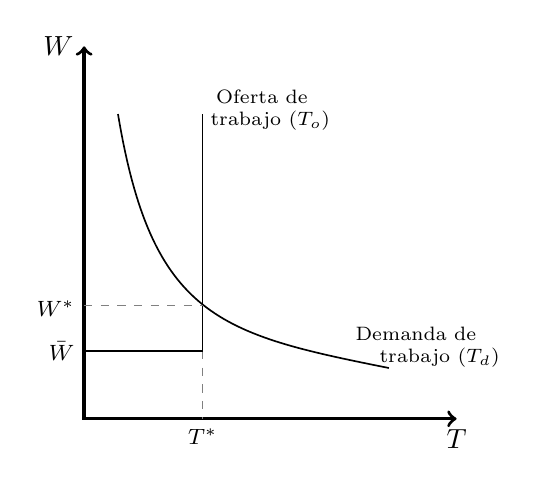
\begin{tikzpicture}[scale=0.43]
\draw[very thick,<->] (0,11) node[left]{$W$}--(0,0)--(11,0) node[below]{$T$};
\draw[semithick] (1,9).. controls (2,3) and (4, 2.5) .. (9, 1.5);
\node [] at (9.8,2.5) {\scriptsize Demanda de};
\node [] at (10.5,1.8) {\scriptsize trabajo ($T_d$)};
\draw[semithick](3.5,2)--(3.5,9);
\draw[thin, dashed, gray] (3.5,2)--(3.5,0);
\node [] at (5.25,9.5) {\scriptsize Oferta de};
\node [] at (5.5,8.8) {\scriptsize  trabajo ($T_o$)};
\node [below] at (3.5,0) {\footnotesize  $T^*$};
\node [left] at (0,3.25) {\footnotesize  $W^*$};
\draw[semithick, dashed,gray] (0,3.35)--(3.5,3.35);
%\draw[semithick, dashed,gray] (0,7)--(3.5,7);
%\draw [semithick,decorate,decoration={brace,amplitude=5pt},xshift=-4pt,yshift=0pt](1.7,7.1) -- (3.6,7.1);
\node [left] at (0,2) {\footnotesize  $\bar{W}$}  ;
\draw[semithick] (0,2)--(3.5,2);
\end{tikzpicture}
\end{center}
\end{figure}

\end{frame}


\begin{frame}{La visión de los Clásicos:  ¿Qué explica el desempleo?}
        \begin{itemize}
          \item \textbf{Desempleo friccional:} es el desempleo que existe incluso en equilibrio, derivado del tiempo que lleva emparejar trabajadores con empleos adecuados.
                \begin{itemize}
                \item Regulaciones laborales que dificultan contrataciones o despidos pueden alargar ese proceso.
                \item La búsqueda de empleo no es inmediata; los trabajadores evalúan ofertas, y las empresas seleccionan cuidadosamente.
                \item La existencia de seguros de desempleo puede reducir la urgencia de aceptar ofertas, prolongando la duración del desempleo friccional.
                \end{itemize}
            \item Salarios de reserva altos: si los trabajadores exigen salarios mínimos elevados por razones culturales, geográficas o familiares, puede haber menos empleos aceptables para ellos.
            \item Problemas de medición: puede clasificarse como desempleado a alguien que en realidad no está buscando activamente o que participa en actividades informales.
        \end{itemize}
\end{frame}

\begin{frame}{La visión Keynesiana}
\vspace{1mm}
    \small El mercado de trabajo \textbf{no siempre} está en equilibrio:
    \begin{itemize}
       \small \item ¿Por qué puede el salario real permanecer fuera del equilibrio?
        \begin{itemize}
         \footnotesize \item Rigideces nominales: no se aceptan reducciones en el salario nominal, incluso si caen los precios.
          \footnotesize  \item Sindicatos: salarios por encima del nivel de equilibrio.
          \footnotesize  \item Contratos de largo plazo: fijan salarios por períodos prolongados.
          \footnotesize  \item Salarios de eficiencia: las empresas pagan salarios superiores al de mercado para incentivar esfuerzo o lealtad.
       \end{itemize}
    \end{itemize}

    \begin{center}
    \begin{figure}[H]
    \begin{center}
    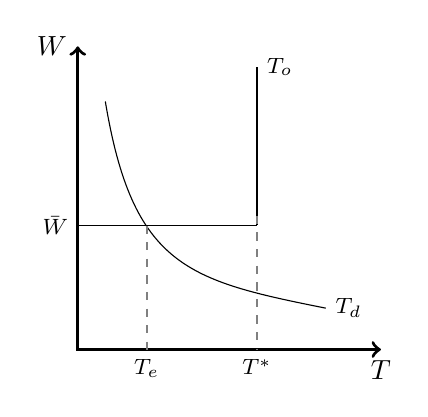
\begin{tikzpicture}[scale=0.35]
    \draw[very thick,<->] (0,11) node[left]{$W$}--(0,0)--(11,0) node[below]{$T$};
    \draw[thin] (1,9).. controls (2,3) and (4, 2.5) .. (9, 1.5) node [right]{\footnotesize $T_d$};
    \draw[thick,gray, dashed](2.5, 4.5)--(2.5, 0);
    \node[below] at (2.5,0) {\footnotesize $T_e$};
    \draw[thick](6.5, 4.5)--(6.5, 10.25) node [right]{\footnotesize $T_o$};
    \draw[thick, gray, dashed] (6.5,4.85)--(6.5,0);
    \node[below] at (6.5,0) {\footnotesize $T^*$};
    \draw[thin](6.5, 4.5)--(0,4.5);
    \node[left] at (0,4.5){\footnotesize $\Bar{W}$};
    \end{tikzpicture}
    \end{center}
    \end{figure}
    \end{center}  
\end{frame}


\begin{frame}{La visión Keynesiana}

\begin{itemize}
    \item ¿Qué pasa si aumentan los precios?
    \item La curva de demanda de trabajo se ubica en una posición más a la derecha, dado que las empresas están
    dispuestas a contratar una mayor cantidad de trabajadores al salario vigente. 
    \item El nivel de empleo alcanzado será mayor
\end{itemize}

    \begin{center}
    \begin{figure}[H]
    \begin{center}
    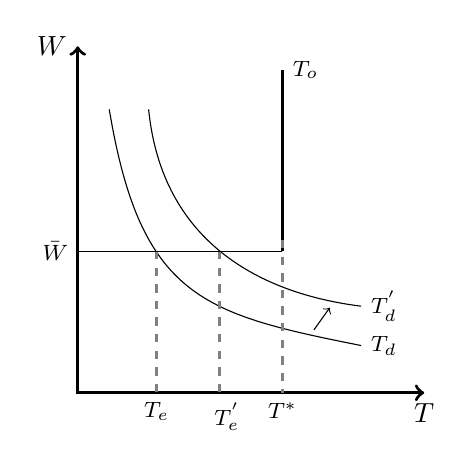
\begin{tikzpicture}[scale=0.4]
    \draw[very thick,<->] (0,11) node[left]{$W$}--(0,0)--(11,0) node[below]{$T$};
    \draw[thin] (1,9).. controls (2,3) and (4, 2.5) .. (9, 1.5) node [right]{\footnotesize $T_d$};
    \draw[thin] (2.25,9).. controls (2.75,4) and (7, 3) .. (9, 2.75) node [right]{\footnotesize $T_d^{'}$};
    \draw[thick,gray, dashed](2.5, 4.5)--(2.5, 0);
    \node[below] at (2.5,0) {\footnotesize $T_e$};
    \draw[thick,gray, dashed](4.5, 4.5)--(4.5, 0);
    \node[below] at (4.75,0) {\footnotesize $T_e^{'}$};
    \draw[thick](6.5, 4.5)--(6.5, 10.25) node [right]{\footnotesize $T_o$};
    \draw[thick, gray, dashed] (6.5,4.85)--(6.5,0);
    \node[below] at (6.5,0) {\footnotesize $T^*$};
    \draw[thin](6.5, 4.5)--(0,4.5);
    \node[left] at (0,4.5){\footnotesize $\Bar{W}$};
    \draw[thin, ->] (7.5,2)--(8,2.7);
    \end{tikzpicture}
    \end{center}
    \end{figure}
    \end{center}  
\end{frame}


\begin{frame}{Midiendo el desempleo}
    \begin{itemize}
    \small \item La EPH (Encuesta Permanente de Hogares) es una de las fuentes de datos más importantes para ver la situación del mercado laboral en Argentina.
    \small  \item Clasificamos a las personas según su relación con el mercado de trabajo:
        \begin{itemize}
            \item Población Económicamente Activa (PEA): personas que \textbf{trabajan} o \textbf{buscan activamente empleo}.
                \[
        \text{PEA} = \text{Empleados}+\text{Desempleados}
                \]
            \item Población Económicamente Inactiva: personas que \textbf{no trabajan ni buscan trabajo}, como estudiantes, jubilados, personas con tareas de cuidado, etc.
        \end{itemize}
        
     \small \item Los cambios en el desempleo pueden deberse no solo a despidos o contrataciones, sino también a movimientos entre la actividad y la inactividad.
        \begin{itemize}
            \item Ejemplo: una persona que estaba inactiva (no buscaba trabajo) comienza a buscar empleo y pasa a ser desempleada, aunque aún no haya sido contratada.
        \end{itemize}
    \end{itemize}
\end{frame}

\begin{frame}{Indicadores básicos del mercado laboral}
    \small
    \begin{itemize}
        \item \textit{Tasa de desempleo}: mide qué porcentaje de la PEA está desempleado.
        \[
        \text{Tasa de desempleo} = \frac{\text{Desempleados}}{\text{PEA}}
        \]
        
        \item \textit{Tasa de empleo}: indica qué parte de la población total está ocupada.
        \[
        \text{Tasa de empleo} = \frac{\text{Empleados}}{\text{Población}}
        \]
        
        \item \textit{Tasa de participación}: mide qué proporción de la población participa activamente del mercado laboral.
        \[
        \text{Tasa de participación} = \frac{\text{PEA}}{\text{Población}}
        \]
        
        \item \textbf{¡Cuidado!} La tasa de desempleo puede subir incluso si más personas consiguen empleo, si al mismo tiempo muchas más personas comienzan a buscar trabajo y se incorporan a la PEA.
    \end{itemize}

\end{frame}

\begin{frame}{¿Puede subir el desempleo aunque aumente el empleo?}
\small
Supongamos una población total de 100 personas.

\textbf{Situación inicial:}
\begin{itemize}
    \item Ocupados: 45 \quad Desempleados: 5 \quad Inactivos: 50
    \item PEA = \pause 45 + 5 = 50
    \item Tasa de desempleo = \pause 5 / 50 = 10\%
\end{itemize}
\textbf{Problema:}
\begin{itemize}
    \item 5 personas inactivas deciden buscar trabajo:
    \begin{itemize}
        \item 3 consiguen empleo $\rightarrow$ ocupados: \pause 48
        \item 2 no consiguen $\rightarrow$ desempleados: \pause 7
    \end{itemize}
    \item Nueva PEA = \pause 48 + 7 = 55
    \item Tasa de desempleo = \pause 7 / 55 $\approx$ 12{,}7\%
\end{itemize}
\textbf{Conclusión:}
\begin{itemize}
    \item Aumentó el empleo (\(+3\)) pero también el desempleo (\(+2\)).
    \item La tasa de desempleo subió, aunque haya más personas trabajando.
\end{itemize}
\end{frame}

\begin{frame}{El mercado de trabajo en la Argentina}
    \centering
    \includegraphics[width=12cm]{Slides Principios de Economia/Figures/Magistral_22/arg_desempleo.png}
\end{frame}

\begin{frame}{La tasa de desempleo en Argentina durante el COVID}
    \centering
    \includegraphics[width=11cm]{Slides Principios de Economia/Figures/Magistral_22/C34.15.jpg}
\end{frame}

\begin{frame}{El mercado de trabajo en la Argentina}
\centering\includegraphics[width=11cm]{Slides Principios de Economia/Figures/Magistral_22/C34.17.jpg}
\end{frame}

\begin{frame}{El mercado de trabajo en la Argentina}
\centering\includegraphics[width=11cm]{Slides Principios de Economia/Figures/Magistral_22/C34.18.jpg}
\end{frame}

\begin{frame}{El mercado de trabajo en la Argentina}
\centering\includegraphics[width=11cm]{Slides Principios de Economia/Figures/Magistral_22/C34.19.jpg}
\end{frame}

\begin{frame}{¿Qué puede pasar con el desempleo en Argentina?}
    \small
    \textbf{Factores que podrían hacer que suba:}
    \begin{itemize}
        \item Estancamiento económico prolongado
        \item Reformas laborales sin incentivos a la contratación
        \item Ajustes fiscales o monetarios contractivos
        \item Caída del consumo interno
    \end{itemize}
    \vspace{0.15cm}
    \textbf{Factores que podrían hacer que baje:}
    \begin{itemize}
        \item Crecimiento sostenido con inversión productiva
        \item Políticas activas de empleo formal
        \item Mejoras en educación y capacitación laboral
    \end{itemize}
    \vspace{0.15cm}
    \textbf{Desafío estructural:}  
    Reducir el desempleo sin aumentar la informalidad. Mejorar la \textit{calidad} del empleo, no solo su cantidad.

    \vspace{0.15cm}
    \textbf{Interrogante:} ¿Y la IA? ¿Cómo afectará al mercado laboral en el futuro?
\end{frame}


\end{document}